\documentclass{article}
\title{On the length of mature microRNAs}
\author{Dave Tang  \\
	RIKEN Yokohama \\
	\and 
	Derek de Rie \\
	VU University Amsterdam \\
	}

\date{\today}

\usepackage{graphicx}
\graphicspath{ {image/} }

\usepackage{hyperref}
\hypersetup{
   colorlinks,
   citecolor=black,
   filecolor=black,
   linkcolor=black,
   urlcolor=black
}

\begin{document}

\maketitle

\begin{abstract}
Despite their size, microRNAs (miRNAs) can have dramatic effects on human health due to their direct effect on transcripts. The misregulation of miRNAs can cause a wide spectrum of diseases, such as cancer, and as such they are under heavily investigation.

\end{abstract}

\section{Introduction}

MicroRNAs (miRNAs) were discovered in 1993\cite{pmid8252621} and are the most well known class of non-coding RNAs (ncRNAs).

\section{Methods and results}\label{method_and_result}

All code underlying this work is available at \url{https://github.com/davetang/mirna_length}. Briefly, random sequences were generated using R (version 3.1.0) and the R Bioconductor package Biostrings\cite{biostrings_package}. We generated three sets of one million random sequences that ranged from 15 to 30 base pairs in length, totalling 48 million sequences. The first two sets of sequences were generated based on the multinomial sequence model where each nucleotide in the sequence is independent and identically distributed. The first set of randomly generated sequences used an equal probability for each nucleotide ($p_{a} = 0.25$, $p_{c} = 0.25$, $p_{g} = 0.25$, $p_{t} = 0.25$). The second set used probabilities based on the what was observed in the human genome (hg38): $p_{a} = 0.29$, $p_{c} = 0.20$, $p_{g} = 0.21$, $p_{t} = 0.30$. The last set of randomly generated sequences used a Markov chain model, where the next sequence depends on the previous sequence. Transitions probabilities (see figure ~\ref{fig:transition}) were derived on dinucleotide frequencies of mature human miRNAs that were downloaded from miRBase\cite{pmid21037258}. The probability of the first base was derived from the frequency of nucleotides at the first base of the human mature miRNAs. The alignment of the sequences was performed using BWA\cite{pmid19451168} (version 0.7.9a-r786) using aln/samse and summaries were created using Perl scripts.

\begin{figure}[h]
   \centering
   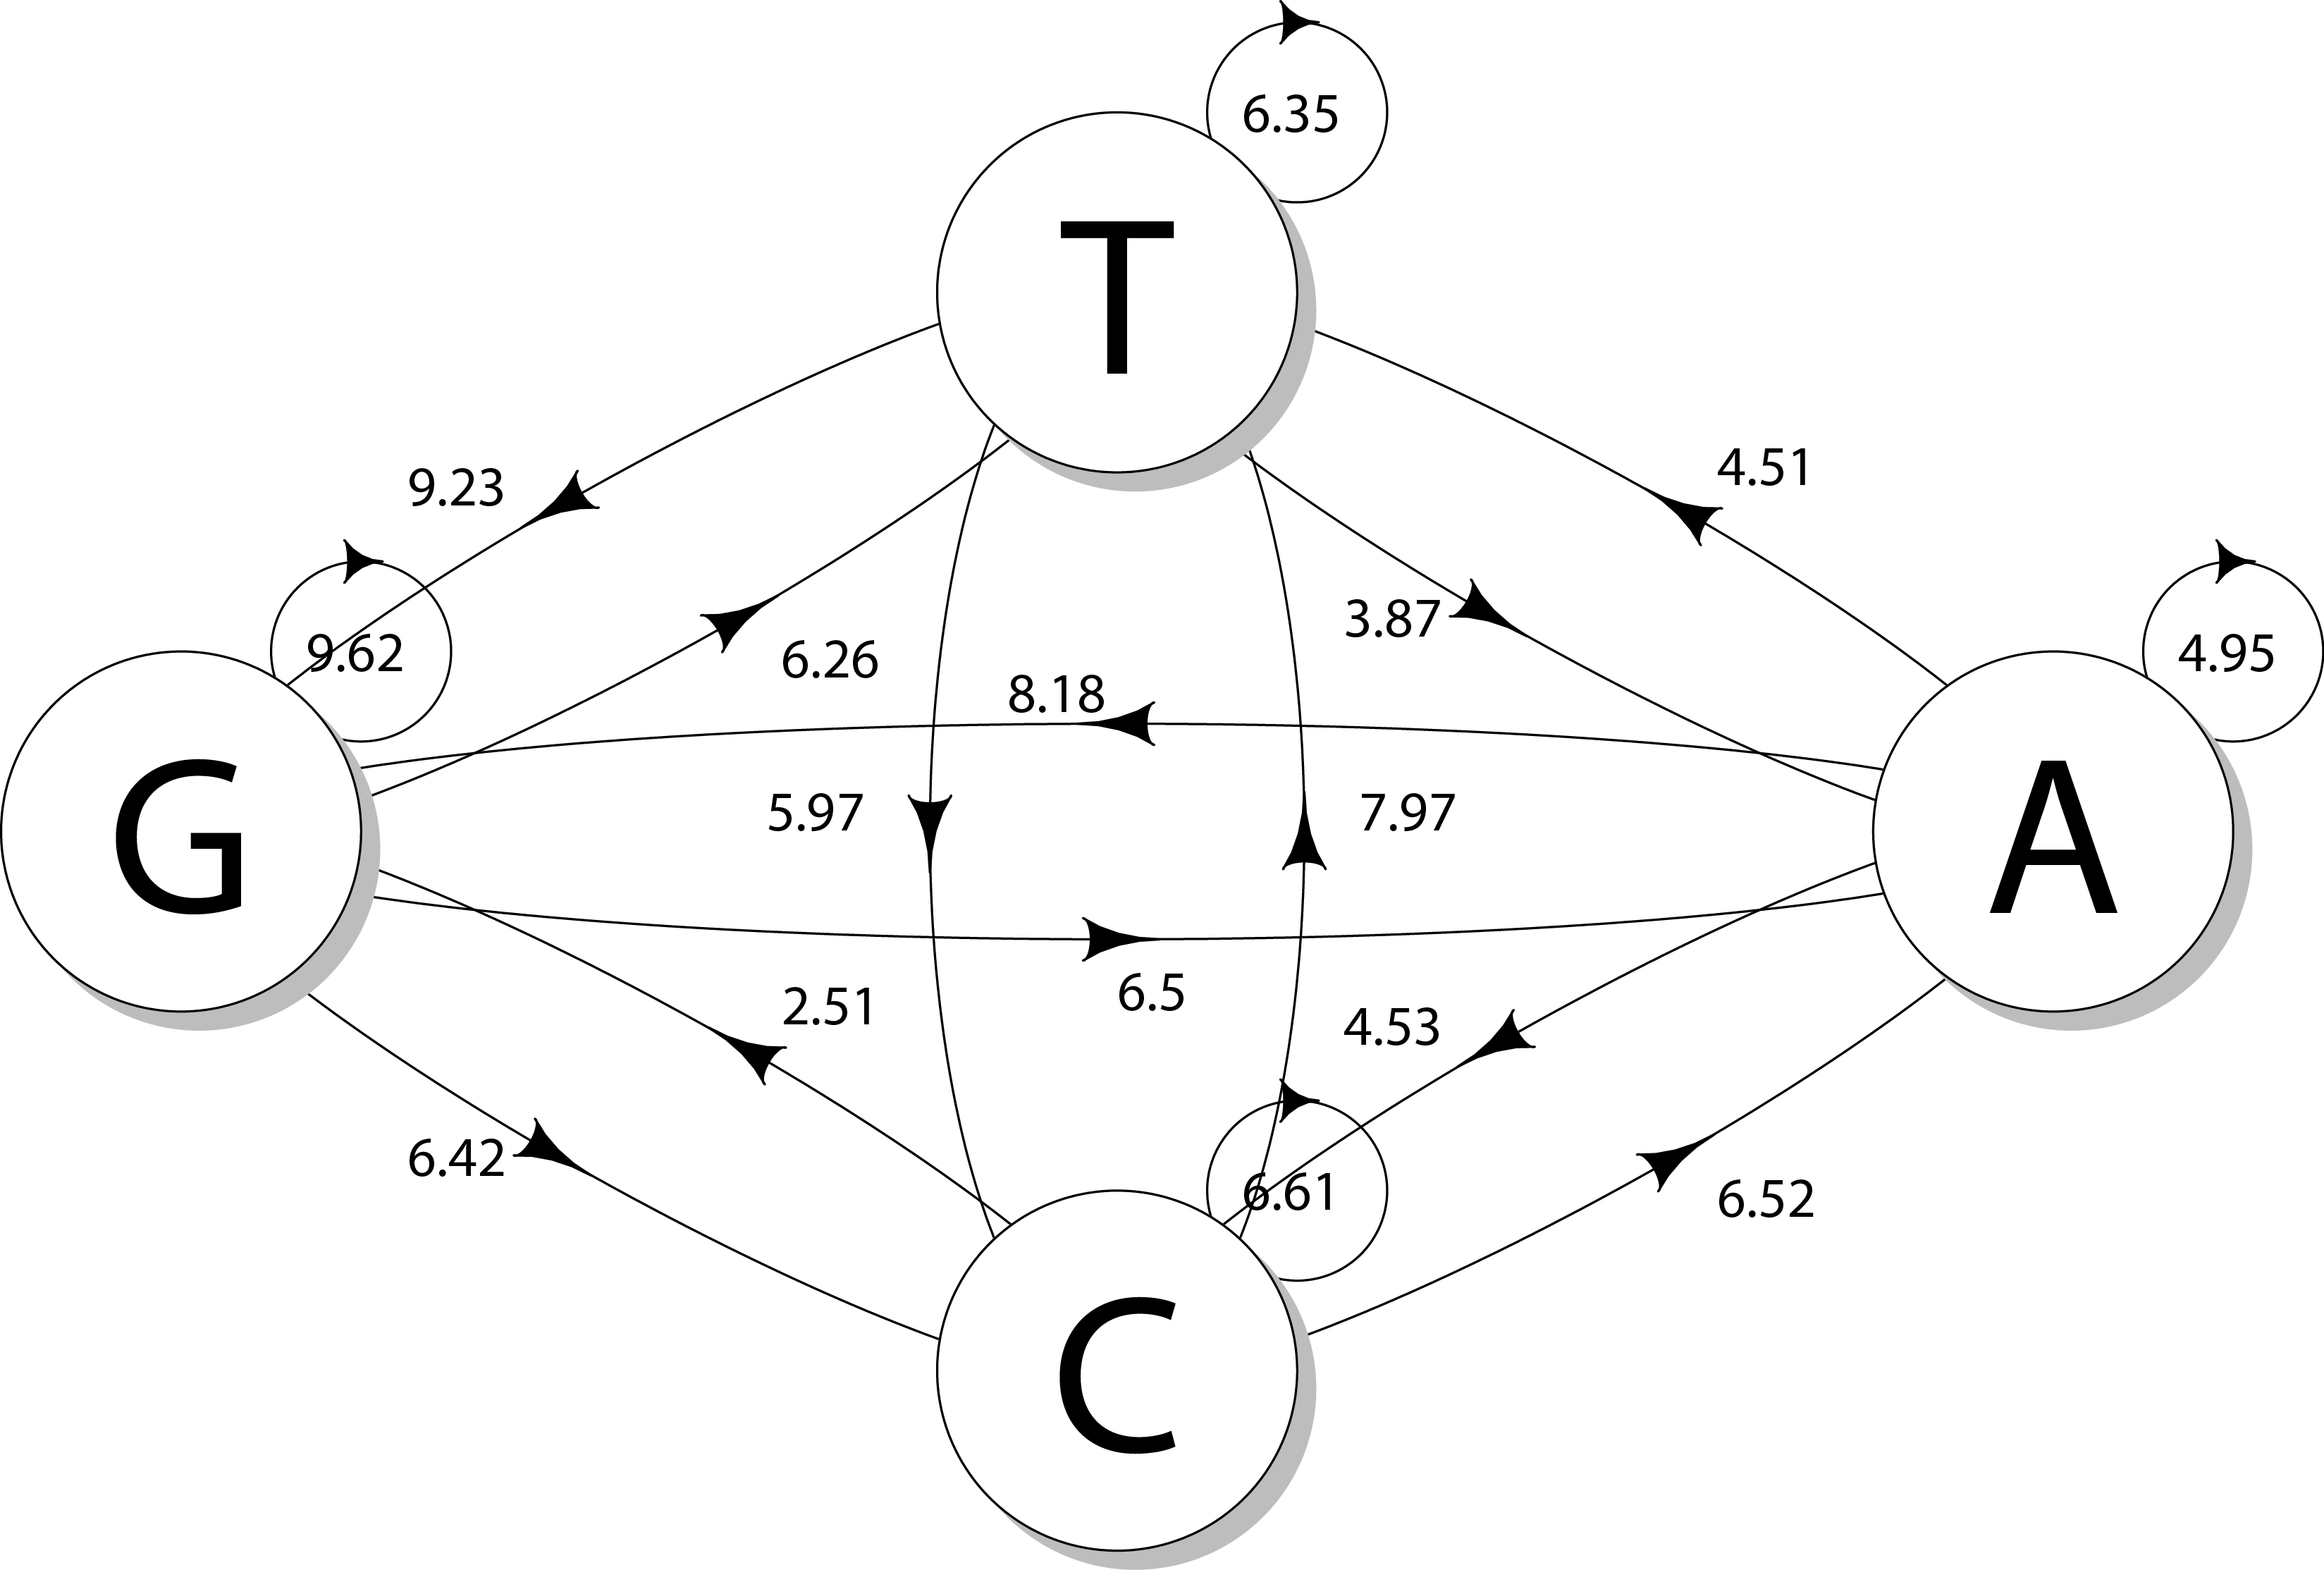
\includegraphics[width=\textwidth,natwidth=3297,natheight=2227]{image/transition.png}
   \caption{Transition diagram based on dinucleotide frequencies of miRBase human miRNAs.}
   \label{fig:transition}
\end{figure}

Bar plot of mapped versus unmapped at each sequence length for the three sets.

Bar plot of perfectly mapped at each sequence length for the three sets.

\section{Discussion}\label{discussion}

\section{Conclusions}\label{conclusion}

Mammalian miRNAs are able to recognise their target miRNA by as little as 6-8 nucleotides; this region is known as the seed region, which lies at the 5' end of a miRNA. However despite this, most miRNAs are 22-23 base pairs in length.

\bibliographystyle{unsrt}
\bibliography{ref}

\end{document}
